% Options for packages loaded elsewhere
\PassOptionsToPackage{unicode}{hyperref}
\PassOptionsToPackage{hyphens}{url}
%
\documentclass[
]{article}
\usepackage{amsmath,amssymb}
\usepackage{iftex}
\ifPDFTeX
  \usepackage[T1]{fontenc}
  \usepackage[utf8]{inputenc}
  \usepackage{textcomp} % provide euro and other symbols
\else % if luatex or xetex
  \usepackage{unicode-math} % this also loads fontspec
  \defaultfontfeatures{Scale=MatchLowercase}
  \defaultfontfeatures[\rmfamily]{Ligatures=TeX,Scale=1}
\fi
\usepackage{lmodern}
\ifPDFTeX\else
  % xetex/luatex font selection
\fi
% Use upquote if available, for straight quotes in verbatim environments
\IfFileExists{upquote.sty}{\usepackage{upquote}}{}
\IfFileExists{microtype.sty}{% use microtype if available
  \usepackage[]{microtype}
  \UseMicrotypeSet[protrusion]{basicmath} % disable protrusion for tt fonts
}{}
\makeatletter
\@ifundefined{KOMAClassName}{% if non-KOMA class
  \IfFileExists{parskip.sty}{%
    \usepackage{parskip}
  }{% else
    \setlength{\parindent}{0pt}
    \setlength{\parskip}{6pt plus 2pt minus 1pt}}
}{% if KOMA class
  \KOMAoptions{parskip=half}}
\makeatother
\usepackage{xcolor}
\usepackage[margin=1in]{geometry}
\usepackage{graphicx}
\makeatletter
\def\maxwidth{\ifdim\Gin@nat@width>\linewidth\linewidth\else\Gin@nat@width\fi}
\def\maxheight{\ifdim\Gin@nat@height>\textheight\textheight\else\Gin@nat@height\fi}
\makeatother
% Scale images if necessary, so that they will not overflow the page
% margins by default, and it is still possible to overwrite the defaults
% using explicit options in \includegraphics[width, height, ...]{}
\setkeys{Gin}{width=\maxwidth,height=\maxheight,keepaspectratio}
% Set default figure placement to htbp
\makeatletter
\def\fps@figure{htbp}
\makeatother
\setlength{\emergencystretch}{3em} % prevent overfull lines
\providecommand{\tightlist}{%
  \setlength{\itemsep}{0pt}\setlength{\parskip}{0pt}}
\setcounter{secnumdepth}{-\maxdimen} % remove section numbering
\ifLuaTeX
  \usepackage{selnolig}  % disable illegal ligatures
\fi
\IfFileExists{bookmark.sty}{\usepackage{bookmark}}{\usepackage{hyperref}}
\IfFileExists{xurl.sty}{\usepackage{xurl}}{} % add URL line breaks if available
\urlstyle{same}
\hypersetup{
  pdftitle={Analysis of RNA-seq data in Alzheimer's Disease Patients},
  pdfauthor={Divya Shridar (Group 2)},
  hidelinks,
  pdfcreator={LaTeX via pandoc}}

\title{Analysis of RNA-seq data in Alzheimer's Disease Patients}
\author{Divya Shridar (Group 2)}
\date{29 Nov 2024}

\begin{document}
\maketitle

{
\setcounter{tocdepth}{2}
\tableofcontents
}
\hypertarget{data-background-and-introduction}{%
\section{Data Background and
Introduction}\label{data-background-and-introduction}}

Scheckel et al.~had explored the role of neuronal ELAV (nELAVL) proteins
in post-mortem Alzheimer's disease (AD) using RNA sequencing data from 9
Alzheimer's patients and 8 controls. In this data set, the sequencing
data is presented as count data of the transcriptome, with 19185 genes
specified. Alongside sequencing data, patient metadata detailing their
age, post-mortem interval, clinical diagnosis rating, plaque values,
CLIP values and sequencing bactch information were found.

As a background, RNA-seq (RNA sequencing) analyzes and quantifies RNA in
a sample, and identifies the types and levels of RNA molecules. This
thus provides insights into gene expression that can contribute to a
better understanding of disease incidence.

From the investigation by Scheckel et al., an increased association
between nELAVL with non-coding Y RNAs during stress, which disrupts
normal mRNA binding and regulation was observed. It is believed that
this could potentially contribute to AD pathology.

\hypertarget{aims}{%
\subsection{Aims}\label{aims}}

This project investigates RNA-seq data from 9 Alzheimer's patients and 8
controls, to find specific genes and proteins that are significantly
associated with an Alzheimer's diagnosis. Additionally, we are
interested in exploring this in the context of patient metadata
information.

\hypertarget{summary-of-findings}{%
\section{Summary of Findings}\label{summary-of-findings}}

\hypertarget{pre-processing}{%
\subsection{Pre-processing}\label{pre-processing}}

As RNA-seq experiments generate relative measurements, normalisation is
required for comparison between samples. In this case, we use the mean
log2 counts-per-million (CPM) to perform quality control on the
sequencing data, while accounting for the batch effect in the processing
of sequencing samples. Low counts of less than 1 were filtered out,
leaving behind 14950 genes. A histogram of normalised CPM counts
reported across all samples can be seen below.

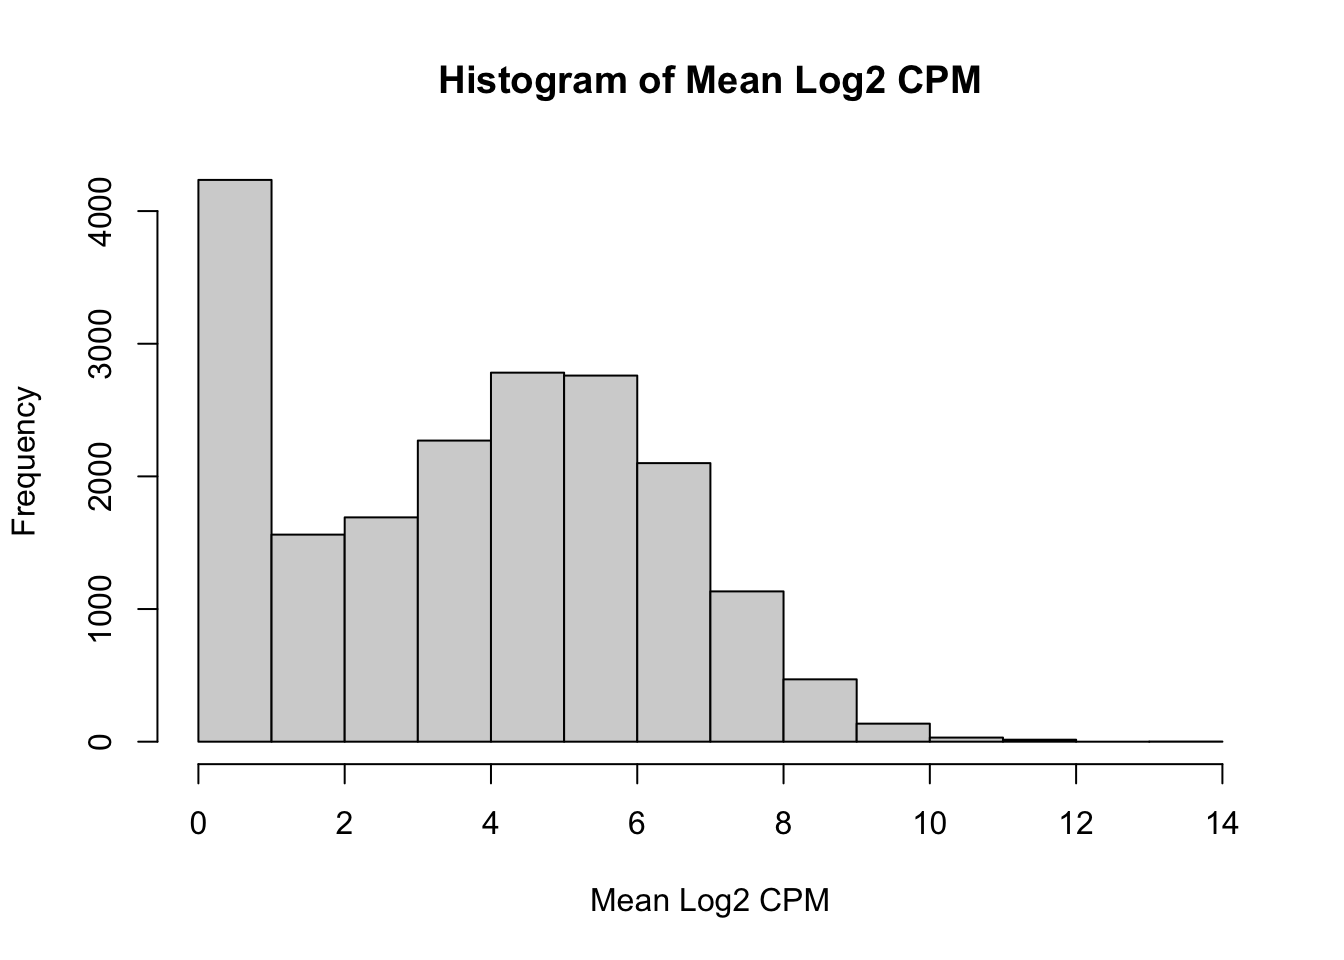
\includegraphics{Divya-s-Report-Template_files/figure-latex/filter low counts using mean log2 CPM-1.pdf}

As it is important to account for differences in transcriptome
composition, library sizes were scaled according to calculated sample
normalisation factors. As count data almost always shows non-trivial
mean-variance relationships, the mean-variance trend for the computed
log2 CPM was estimated, before being used to compute appropriate
observation-level weights based on the predicted variance. The end goal
is to ensure the data is ready for linear modelling as the weights are
used to adjust for heteroscedasticity. The new data distribution after
normalisation is seen below.

\includegraphics{Divya-s-Report-Template_files/figure-latex/unnamed-chunk-2-1.pdf}

Using Spearman correlation, the correlation between the different
patient conditions were analysed using their now normalised count
information. This was visualised with the heatmap seen below.

\includegraphics{Divya-s-Report-Template_files/figure-latex/unnamed-chunk-3-1.pdf}

Principal Component Analysis (PCA) was also performed on the normalised
data, in relation to patient condition.

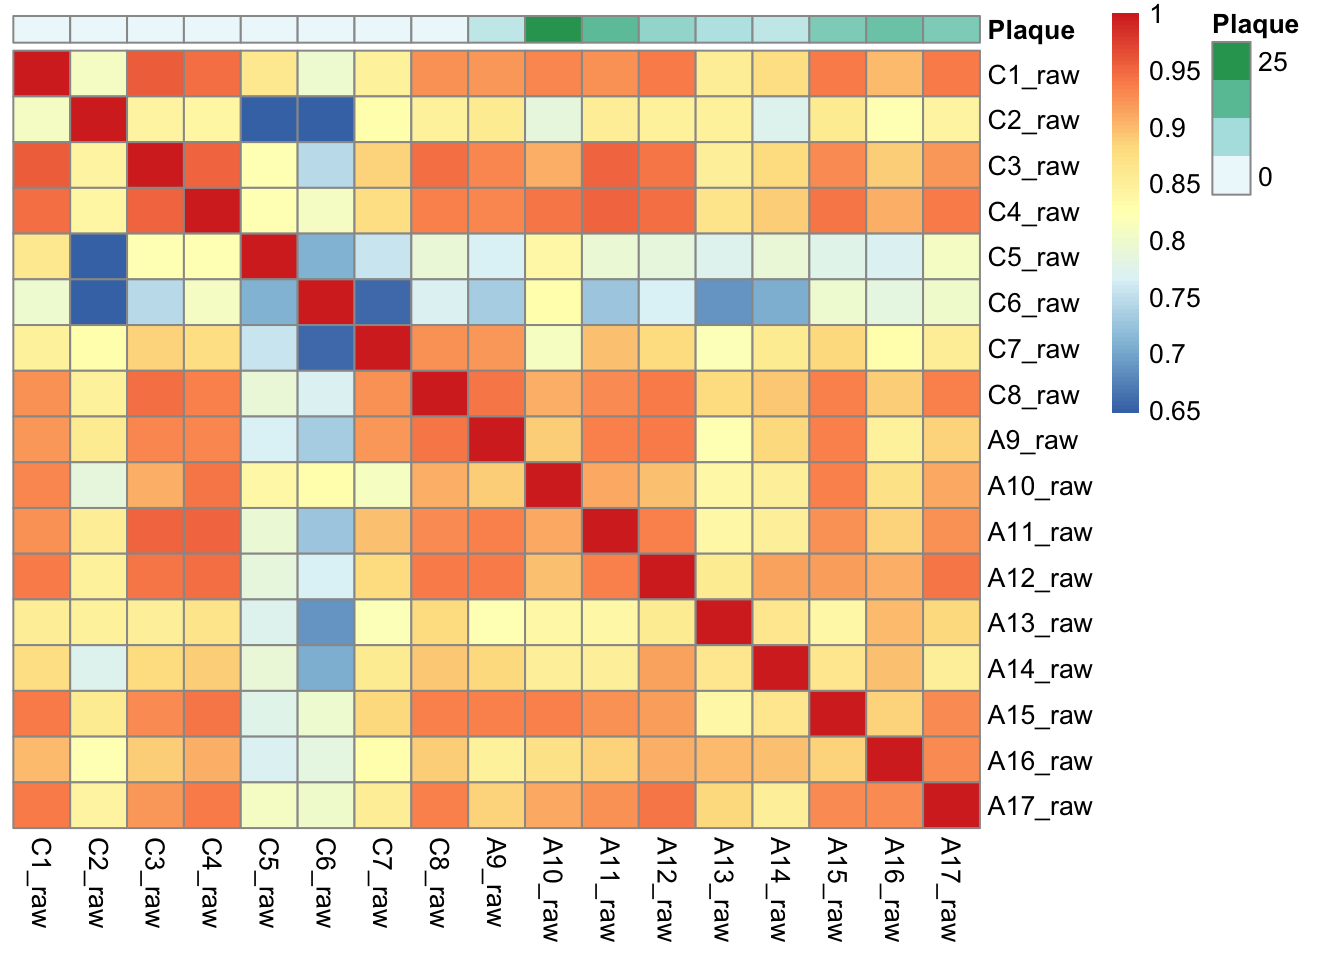
\includegraphics{Divya-s-Report-Template_files/figure-latex/unnamed-chunk-4-1.pdf}

At this point, the Alzheimers patient cluster appears to be close
together. However, the controls appear to be lying far out (see C2, C5
and C6), or in the centre of the cluster of Alzheimers patients (see
C1).

We then also evaluted the correlation between the sequencing batch
information and normalised count data. The resultant heatmap and PCA
plots can be seen below.

\includegraphics{Divya-s-Report-Template_files/figure-latex/QC: batch heatmap-1.pdf}

\includegraphics{Divya-s-Report-Template_files/figure-latex/QC: PCA by Batch-1.pdf}

At this stage, data points C1, C5 and C6 were removed from further
analysis as they had been identified as outliers.

Presentation Feedback! This performed PCA should not have led to outlier
removal, and it would have been better to maintain all data points due
to the small sample size.

\hypertarget{gene-disease-exploration}{%
\subsection{Gene-Disease Exploration}\label{gene-disease-exploration}}

\hypertarget{protein-disease-exploration}{%
\subsection{Protein-Disease
Exploration}\label{protein-disease-exploration}}

\hypertarget{patient-disease-exploration}{%
\subsection{Patient-Disease
Exploration}\label{patient-disease-exploration}}

\begin{enumerate}
\def\labelenumi{\arabic{enumi}.}
\tightlist
\item
  Item 1
\item
  Item 2
\item
  Item 3

  \begin{itemize}
  \tightlist
  \item
    Item 3a
  \item
    Item 3b
  \end{itemize}
\end{enumerate}

\hypertarget{reflections}{%
\section{Reflections}\label{reflections}}

\hypertarget{statistical-challenges-related-to-this-work-proposed-design-and-method-choice}{%
\subsection{Statistical challenges related to this work; Proposed Design
and Method
Choice}\label{statistical-challenges-related-to-this-work-proposed-design-and-method-choice}}

\end{document}
